\newenvironment{QandA}{\begin{enumerate}[label=\bfseries\alph*.]\bfseries}
        {\end{enumerate}}
\newenvironment{answered}{\par\normalfont}{}

\chapter{Case Study}\label{ch:case-study}

In December 2019, a virus known as COVID-19 was first identified in Wuhan, China~\cite{seznam-korona2021}.
Three months later, on March 1, 2020, the first three cases of the disease were confirmed in the Czech Republic~\cite{seznam-korona2021}.
The disease has shown and continues to show the shortcomings of social and political environment worldwide.
But the disease, although very serious, has given us many opportunities.
One such opportunity is open datasets made available by state institutions.

In the following part of the work we will try to analyze the state of datasets provided by the institutions of the Czech Republic.
We apply the metrics defined in Chapter 3 to the data in order to objectively measure their quality and comment on the results.
Available datasets as of April 1, 2020 from the URL address \url{https://onemocneni-aktualne.mzcr.cz/} are listed in Appendix~\ref{ch:dataset-collection}.

\section{Technical Analysis}

The data can be downloaded via the REST API in JSON, in addition, the data can be downloaded in CSV together with metadata also in JSON format.
The format of the JSON data file can be seen in Figure~\ref{ls:data}.
All data files contain one main object, with three keys (modified, source and data).
The \enquote{modified} key contains the date of the dataset update in ISO 8601 format with the time offset from UTC (Coordinated Universal Time).
The \enquote{source} key contains the URL of the dataset, especially the protocol and domain name.
The last key, the data, contains an array of json objects with a structure given by the metadata.
This is an array of objects even if the array contains only one object.

\begin{figure}[htb]
    \centering

    \begin{lstlisting}[language=json,firstnumber=1]
{
    "modified": "2021-04-18T12:28:42+02:00",
    "source": "https:\/\/onemocneni-aktualne.mzcr.cz\/",
    "data": [
        {
            ...
        }
    ]
}
    \end{lstlisting}

    \caption{Data file structure}
    \label{ls:data}
\end{figure}
\FloatBarrier

An example of the structure of the metadata file can be found in the appendix~\ref{ch:metadata-file-structure}.

\section{Data Quality Analysis}

Long et al. (2004) wrote a comprehesive data quality checklist for emergency medical services data~\cite{long2004}.
We will use this checklist as a base for our own data evaluation.

\subsection{Relevance}

\begin{table}[htbp]
    \centering

    %\begin{tabular}{@{}llrrrrrrrrrr@{}}
    \begin{tabular}{llrrrrrrrrrr}
        \toprule
        \multirow{2}{*}{Dimensions} & \multirow{2}{*}{Characteristics}  & \multicolumn{10}{c}{Criteria}         \\ \cmidrule(lr){3-12}
                                    &                                   & a & b & c & d & e & f & g & h & i & j \\ \midrule
        \multirow{2}{*}{Relevance}  & Adaptability                      & 2 & 2 & 2 & 0 & 2 & 0 & 2 & 0 & 2 &   \\
                                    & Value                             & 2 & 0 &   &   &   &   &   &   &   &   \\
        \bottomrule
    \end{tabular}

    \caption{Evaluation of criteria for dimension Relevance}
    \label{table:relevance-benchmark}
\end{table}
\FloatBarrier

\subsubsection{Value}

\begin{QandA}
    \item The purpose of the data is clear.
    \begin{answered}
        Yes, the general purpose of the data is obvious.
        The data is provided by the Institute of Health Information and Statistics of the Czech Republic.
        Individual datasets have a description that specifies their purpose.
    \end{answered}

    \item The data shed light on the issues of most importance to users and the data are used in policy formulation and decision making.
    \begin{answered}
        Yes, the data provide information on the current development of the epidemic situation in the Czech Republic.
        The dynamics of the \textit{Compartmental Model} can be derived from the data and thus predictive analysis can be done.
        The data are used for policy formulation and decision making.
    \end{answered}

    \item There are no other more valid sources for the data.
    \begin{answered}
        Yes, the data is provided by a government agency.
        There is no other source of data for the public.
    \end{answered}

    \item Client liaison mechanisms are in place and client needs are monitored.
    \begin{answered}
        Unknown.
    \end{answered}

    \item How the data are used is known and well understood.
    \begin{answered}
        The Institute of Health Information and Statistics of the Czech Republic publishes summaries of the epidemiological situation and other reports, including descriptions of methodologies for using data for predictions.
        Formally, this point is met.
    \end{answered}

    \item Client evaluations are conducted and reviewed.
    \begin{answered}
        Unknown.
    \end{answered}

    \item The data are found to meet the needs of its users.
    \begin{answered}
        In this case, as \enquote{needs of the users} is considered the awareness of the general public.
        From this point of view, the question is met.
    \end{answered}

    \item Client evaluations are conducted and reviewed.
    \begin{answered}
        During the publication of datasets, many modifications and additions were made.
        Feedback taken into account.
        However, we do not have information to what extent.
        The point is therefore classified as \textbf{unknown}.
    \end{answered}

    \item The data are found to be worth the resources dedicated to its production.
    \begin{answered}
        Yes, these data are necessary to inform the public about the current state of development of the pandemic.
        Almost any expenditure is worthwhile in this case.
    \end{answered}

\end{QandA}

\subsubsection{Adaptability}

\begin{QandA}
    \item The data can be used to inform emerging issues and can adapt to change.
    \begin{answered}
        Yes, this has been demonstrated in the past by the introduction of anti-epidemic measures and the changes that have been introduced in the datasets.
    \end{answered}

    \item Ongoing explicit program review and priority determination are conducted.
    \begin{answered}
        The degree of review by the data issuer is \textbf{unknown}.
    \end{answered}

\end{QandA}

\subsection{Accuracy}

\begin{table}[htbp]
    \centering

    %\begin{tabular}{@{}llrrrrrrrrrr@{}}
    \begin{tabular}{llrrrrrrrrrr}
        \toprule
        \multirow{2}{*}{Dimensions} & \multirow{2}{*}{Characteristics}  & \multicolumn{10}{c}{Criteria}         \\ \cmidrule(lr){3-12}
                                    &                                   & a & b & c & d & e & f & g & h & i & j \\ \midrule
        \multirow{13}{*}{Accuracy}  & Form Design and Completion        &   &   &   &   &   &   &   &   &   &   \\
                                    & Frame                             &   &   &   &   &   &   &   &   &   &   \\
                                    & Over Coverage                     &   &   &   &   &   &   &   &   &   &   \\
                                    & Under Coverage                    &   &   &   &   &   &   &   &   &   &   \\
                                    & Response                          &   &   &   &   &   &   &   &   &   &   \\
                                    & Completeness                      &   &   &   &   &   &   &   &   &   &   \\
                                    & Bias                              &   &   &   &   &   &   &   &   &   &   \\
                                    & Validity                          &   &   &   &   &   &   &   &   &   &   \\
                                    & Reliability                       &   &   &   &   &   &   &   &   &   &   \\
                                    & Collection                        &   &   &   &   &   &   &   &   &   &   \\
                                    & Processing                        &   &   &   &   &   &   &   &   &   &   \\
                                    & Imputation                        &   &   &   &   &   &   &   &   &   &   \\
                                    & Analysis                          &   &   &   &   &   &   &   &   &   &   \\
        \bottomrule
    \end{tabular}

    \caption{Evaluation of criteria for dimension Accuracy}
    \label{table:accuracy-benchmark}
\end{table}
\FloatBarrier

\subsubsection{Form Design and Completion}

\begin{QandA}
    \item The data retrieval form was designed by a team that includes methodologists, a form design expert, representatives for those who are responsible for completing the form, as well as other subject matter experts.
    \begin{answered}
        
    \end{answered}

    \item The purpose and population of interest are clear and well documented.
    \begin{answered}
        
    \end{answered}

    \item There is adequate justification for each field gathered.
    \begin{answered}
        
    \end{answered}

    \item The form is user-friendly and is accompanied by a clear, readily accessible, and user-friendly manual that describes in detail the data collection guidelines including when and how to complete the form and defines each field in detail.
    \begin{answered}
        
    \end{answered}

    \item Those responsible for completing the form receive training so that they are able to properly complete the form.
    \begin{answered}
        
    \end{answered}

    \item As part of training, the importance of the data is conveyed and those responsible for completing the form are tested and immediate feedback is provided regarding the reliability and validity of their performance.
    \begin{answered}
        
    \end{answered}

    \item Those responsible for completing the form are allocated the time and have the motivation to do so, as well as confidence in the form completion process.
    \begin{answered}
        
    \end{answered}

    \item The data are monitored for outliers, logical errors, completeness, and consistency and ongoing monitoring and constructive feedback is provided to the primary collectors where necessary.
    \begin{answered}
        
    \end{answered}

    \item Any major revisions to the original form design (purpose, structure, etc.) of the database and the dates of any major revisions are known, documented, and readily available. Moreover, an explicit consideration of overall trade-offs between accuracy, cost, timeliness, and respondent burden was conducted at the design stage.
    \begin{answered}
        
    \end{answered}

    \item A revised form is pilot tested until high standards of reliability and validity are met and the pilot test results are readily available.
    \begin{answered}
        
    \end{answered}

\end{QandA}

\subsubsection{Frame}

\begin{QandA}
    \item The frame is known and documented.
    \begin{answered}
        
    \end{answered}

    \item The frame is maintained in an ongoing manner.
    \begin{answered}
        
    \end{answered}

\end{QandA}

\subsubsection{Over Coverage}

\begin{QandA}
    \item Only qualifying data suppliers are on the frame.
    \begin{answered}
        
    \end{answered}

    \item The data are checked for duplicates and erroneous entries from qualifying suppliers.
    \begin{answered}
        
    \end{answered}

\end{QandA}

\subsubsection{Under Coverage}

\begin{QandA}
    \item Data are received from all qualifying data suppliers on the frame.
    \begin{answered}
        
    \end{answered}

    \item The list of those actually sending data are compared to independent lists.
    \begin{answered}
        
    \end{answered}

\end{QandA}

\subsubsection{Response}

\begin{QandA}
    \item The overall expected and actually received number of records are known and tracked per year and response across month is checked and compared against previous years.
    \begin{answered}
        
    \end{answered}

    \item The amount of missing data per record is known and tracked per field per year and key fields (e.g., age, gender, and clinical code) are at least 98\% complete.
    \begin{answered}
        
    \end{answered}

\end{QandA}

\subsubsection{Completeness}

\begin{QandA}
    \item The patient service form/chart used for data retrieval form abstraction is easy to understand.
    \begin{answered}
        
    \end{answered}

    \item The form/chart used for abstraction is complete.
    \begin{answered}
        
    \end{answered}

    \item All patient encounters/visits are abstracted and represented in the database.
    \begin{answered}
        
    \end{answered}

    \item All fields are systematically completed per patient record.
    \begin{answered}
        
    \end{answered}

\end{QandA}

\subsubsection{Bias}

\begin{QandA}
    \item Explicit standard guidelines are in place and adherence is monitored for data collection
    \begin{answered}
        
    \end{answered}

    \item Clear guidelines and training eliminate as much as possible the need for interpretation.
    \begin{answered}
        
    \end{answered}

    \item For data that need to be classified, clear coding standards are available.
    \begin{answered}
        
    \end{answered}

    \item For data that need to be classified, the available standards are adhered to.
    \begin{answered}
        
    \end{answered}

    \item For data that need to be classified, only highly trained certified staff classify the data.
    \begin{answered}
        
    \end{answered}

    \item Sources of bias (e.g., upcoding) are understood and eliminated if possible and ongoing quality assurance tests ensure that data collection, abstraction, and entry are conducted in a standard manner according to guidelines.
    \begin{answered}
        
    \end{answered}

\end{QandA}

\subsubsection{Validity}

\begin{QandA}
    \item The patient service form/chart is complete and reflects the patient encounter and the codesheet or abstract that is based on the form/chart reflects what is in the form/chart.
    \begin{answered}
        
    \end{answered}

    \item Adequate resources are in place to ensure valid timely data and ongoing database improvement.
    \begin{answered}
        
    \end{answered}

    \item Random audits and/or reabstraction studies are conducted and the data are compared to external sources of the same or similar data (if possible).
    \begin{answered}
        
    \end{answered}

    \item Validity coefficients are available and are greater than or equal to 0.8 for key data elements (i.e., postal code, patient age, most responsible diagnosis, procedures, and comorbities).
    \begin{answered}
        
    \end{answered}

\end{QandA}

\subsubsection{Reliability}

\begin{QandA}
    \item Reliability studies of key data elements (e.g., age, gender, and clinical code) are conducted at regular intervals.
    \begin{answered}
        
    \end{answered}

    \item Intra rater coefficients are available.
    \begin{answered}
        
    \end{answered}

    \item Inter rater coefficients are available.
    \begin{answered}
        
    \end{answered}

    \item Rater coefficients are greater than or equal to 0.8 for key data elements (i.e., postal code, patient age, most responsible diagnosis, procedures, and comorbities).
    \begin{answered}
        
    \end{answered}

\end{QandA}

\subsubsection{Collection}

\begin{QandA}
    \item Standard data retrieval form is in place.
    \begin{answered}
        
    \end{answered}

    \item Range checks are place for all fields at data entry and key logic checks are run (e.g., checks for clinical impossibilities or date of birth greater than call date).    
    \begin{answered}
        
    \end{answered}

    \item Standard data specifications are provided to vendor(s).
    \begin{answered}
        
    \end{answered}

    \item Standard test data are used to test edits.
    \begin{answered}
        
    \end{answered}

    \item Data entry software and equipment are user friendly.
    \begin{answered}
        
    \end{answered}

    \item Staff is available and motivated to enter the data and data entry is monitored and constructive feedback is provide to staff.
    \begin{answered}
        
    \end{answered}

    \item Edit errors are set aside and made available for analysis.
    \begin{answered}
        
    \end{answered}

    \item Data entry of abstracted data takes place in close proximity to the original data (original forms/charts).
    \begin{answered}
        
    \end{answered}

    \item Error detection reports are generated.
    \begin{answered}
        
    \end{answered}

    \item Error correction is documented.
    \begin{answered}
        
    \end{answered}

\end{QandA}

\subsubsection{Processing}

\begin{QandA}
    \item All programming is tested and the results are documented.
    \begin{answered}
        
    \end{answered}

    \item Ongoing quality control checks are conducted on electronically extracted data.
    \begin{answered}
        
    \end{answered}

    \item Documentation on how the various systems involved interact, extract, change, and/or append the data exists and is available.
    \begin{answered}
        
    \end{answered}

    \item Ongoing tests are run to ensure all systems are interacting properly.
    \begin{answered}
        
    \end{answered}

\end{QandA}

\subsubsection{Imputation}

\begin{QandA}
    \item Imputation is automatically derived.
    \begin{answered}
        
    \end{answered}

    \item The raw data are preserved.
    \begin{answered}
        
    \end{answered}

\end{QandA}

\subsubsection{Analysis}

\begin{QandA}
    \item Edit errors are analyzed.
    \begin{answered}
        
    \end{answered}

    \item Error detection analyses are conducted and the data are checked for missing data.
    \begin{answered}
        
    \end{answered}

    \item Outliers or other suspicious data are investigated.
    \begin{answered}
        
    \end{answered}

    \item Regular standard summary analyses are conducted and made available.
    \begin{answered}
        
    \end{answered}

\end{QandA}

\subsection{Timeliness}

\begin{table}[htbp]
    \centering

    %\begin{tabular}{@{}llrrrrrrrrrr@{}}
    \begin{tabular}{llrrrrrrrrrr}
        \toprule
        \multirow{2}{*}{Dimensions} & \multirow{2}{*}{Characteristics}  & \multicolumn{10}{c}{Criteria}         \\ \cmidrule(lr){3-12}
                                    &                                   & a & b & c & d & e & f & g & h & i & j \\ \midrule
        \multirow{2}{*}{Timeliness}   & Data Currency                     &   &   &   &   &   &   &   &   &   &   \\
                                    & System Efficiency                 &   &   &   &   &   &   &   &   &   &   \\
        \bottomrule
    \end{tabular}

    \caption{Evaluation of criteria for dimension Timeliness}
    \label{table:timeliness-benchmark}
\end{table}
\FloatBarrier

\subsubsection{Data Currency}

\begin{QandA}
    \item The time between original form or chart completion and data abstraction is reasonably brief.
    \begin{answered}
        
    \end{answered}

    \item The time between the end of the reference period to which the data pertain and data release is reasonably brief.
    \begin{answered}
        
    \end{answered}

    \item The official date of release was announced in advance of the release.
    \begin{answered}
        
    \end{answered}

    \item The official date of release was achieved.
    \begin{answered}
        
    \end{answered}

\end{QandA}

\subsubsection{System Efficiency}

\begin{QandA}
    \item Database methods are regularly reviewed for efficiency.
    \begin{answered}
        
    \end{answered}

    \item Processing methods are regularly reviewed for efficiency.
    \begin{answered}
        
    \end{answered}

\end{QandA}

\subsection{Accessibility}

\begin{table}[htbp]
    \centering

    %\begin{tabular}{@{}llrrrrrrrrrr@{}}
    \begin{tabular}{llrrrrrrrrrr}
        \toprule
        \multirow{2}{*}{Dimensions}     & \multirow{2}{*}{Characteristics}  & \multicolumn{10}{c}{Criteria}         \\ \cmidrule(lr){3-12}
                                        &                                   & a & b & c & d & e & f & g & h & i & j \\ \midrule
        \multirow{2}{*}{Accessibility}  & Awareness                         &   &   &   &   &   &   &   &   &   &   \\
                                        & Ease of Access                    &   &   &   &   &   &   &   &   &   &   \\
        \bottomrule
    \end{tabular}

    \caption{Evaluation of criteria for dimension Accessibility}
    \label{table:accessibility-benchmark}
\end{table}
\FloatBarrier

\subsubsection{Awareness}

\begin{QandA}
    \item The existence of the data can be ascertained.
    \begin{answered}
        
    \end{answered}

    \item Standard tables and analyses are produced and made available per reference period.
    \begin{answered}
        
    \end{answered}

\end{QandA}

\subsubsection{Ease of Access}

\begin{QandA}
    \item The data are well organized and readily available for users.
    \begin{answered}
        
    \end{answered}

    \item Privacy and confidentiality rules related to accessibility are adhered to.
    \begin{answered}
        
    \end{answered}

\end{QandA}

\subsection{Interpretability}

\begin{table}[htbp]
    \centering

    %\begin{tabular}{@{}llrrrrrrrrrr@{}}
    \begin{tabular}{llrrrrrrrrrr}
        \toprule
        \multirow{2}{*}{Dimensions}         & \multirow{2}{*}{Characteristics}  & \multicolumn{10}{c}{Criteria}         \\ \cmidrule(lr){3-12}
                                            &                                   & a & b & c & d & e & f & g & h & i & j \\ \midrule
        \multirow{2}{*}{Interpretability}   & Documentation                     &   &   &   &   &   &   &   &   &   &   \\
                                            & Education                         &   &   &   &   &   &   &   &   &   &   \\
        \bottomrule
    \end{tabular}

    \caption{Evaluation of criteria for dimension Interpretability}
    \label{table:interpretability-benchmark}
\end{table}
\FloatBarrier

\subsubsection{Documentation}

\begin{QandA}
    \item The limitations of the data are documented for users using a standard format and the documentation is readily available for users.
    \begin{answered}
        
    \end{answered}

    \item The supplementary information and metadata necessary to interpret and utilize the data appropriately are kept up to date and are readily available.
    \begin{answered}
        
    \end{answered}

\end{QandA}

\subsubsection{Education}

\begin{QandA}
    \item Examples of how the data can be used appropriately are provided.
    \begin{answered}
        
    \end{answered}

    \item Staff is available to answer questions about the data and to aid interpretation.
    \begin{answered}
        
    \end{answered}

\end{QandA}

\subsection{Coherence}

\begin{table}[htbp]
    \centering

    %\begin{tabular}{@{}llrrrrrrrrrr@{}}
    \begin{tabular}{llrrrrrrrrrr}
        \toprule
        \multirow{2}{*}{Dimensions} & \multirow{2}{*}{Characteristics}  & \multicolumn{10}{c}{Criteria}         \\ \cmidrule(lr){3-12}
                                    &                                   & a & b & c & d & e & f & g & h & i & j \\ \midrule
        \multirow{3}{*}{Coherence}  & Standardization                   &   &   &   &   &   &   &   &   &   &   \\
                                    & Linkage                           &   &   &   &   &   &   &   &   &   &   \\
                                    & Historical Comparability          &   &   &   &   &   &   &   &   &   &   \\
        \bottomrule
    \end{tabular}

    \caption{Evaluation of criteria for dimension Coherence}
    \label{table:coherence-benchmark}
\end{table}
\FloatBarrier

\subsubsection{Standardization}

\begin{QandA}
    \item All data elements are compared to a standard data dictionary in an ongoing manner and for classified data, standard classification methodologies are used (e.g., ICD10).
    \begin{answered}
        
    \end{answered}

    \item As many data elements as possible conform to a standard data dictionary.
    \begin{answered}
        
    \end{answered}

    \item Data are collected at the finest level of detail as is practical.
    \begin{answered}
        
    \end{answered}

    \item For any derived variable, the original variable or variables are also maintained.
    \begin{answered}
        
    \end{answered}

\end{QandA}

\subsubsection{Linkage}

\begin{QandA}
    \item Standard Geographical Classifications (SGC) can be used.
    \begin{answered}
        
    \end{answered}

    \item Data are collected using a consistent time frame (e.g., fiscal year).
    \begin{answered}
        
    \end{answered}

    \item Codes are used to uniquely identify institutions (e.g., hospital numbers) and persons (e.g., health insurance number).
    \begin{answered}
        
    \end{answered}

    \item Privacy and confidentiality rules related to record linkage are adhered to.
    \begin{answered}
        
    \end{answered}

\end{QandA}

\subsubsection{Historical Comparability}

\begin{QandA}
    \item Trend analysis is used to examine changes in key data elements over time and breaks in the series are explained.
    \begin{answered}
        
    \end{answered}

    \item Documentation of changes in concepts or methods exists and is readily accessible.
    \begin{answered}
        
    \end{answered}

\end{QandA}

One of the most serious errors in the data catalog is the absence of categorization of deaths.
% V datasetu, obsahujícím data o úmrtí pacientů, se dozvíme datum úmrtí, věk pacienta, pohlaví a kódy kraje a obce ze kterého pacient pocházel.
In the dataset, which contains data on patients' deaths, we learn the date of death, the patient's age, gender and the codes of the region and municipality from which the patient came.
It does not take into account whether the patient was very ill (e.g., a patient with pancreatic cancer in advanced metastasis) or generally polymorbid (i.e., having number of illnesses) and therefore had a high probability of death, or if the patient was a completely healthy person.
No consideration of this fact leads to the introduction of virtually immeasurable systematic error.

\begin{figure}[htb]
    \centering

    \begin{lstlisting}[language=json,firstnumber=1]
[
    {
    "datum": "2020-01-01",
    "vek": 50,
    "pohlavi": "M",
    "kraj_nuts_kod": "CZ000",
    "okres_lau_kod": "CZ0000"
    },...
]
    \end{lstlisting}

    \caption{Sample data with information on deceased patients}
    \label{ls:sample-data-deceased}
\end{figure}
\FloatBarrier

A similar issue can be observed in the data on new COVID-19 cases and the daily number of tests performed.
In the first case we are unable to determine whether there are any percentage of patients in whom the disease manifested itself repeatedly.
In the second case, information on retested patients is missing, as well as information on whether the tested patient showed symptoms of the disease.
All these problems lead to a reduction in data quality, which we are not able to measure effectively.

Another factor reducing the quality is the methodology itself.
According to the methodology, a person is considered cured since the last negative test.
However, it does not take into account whether this person is still in the \textit{Intensive Care Unit} with post-COVID syndrome or whether he is really cured.

\begin{figure}[htb]
    \centering
    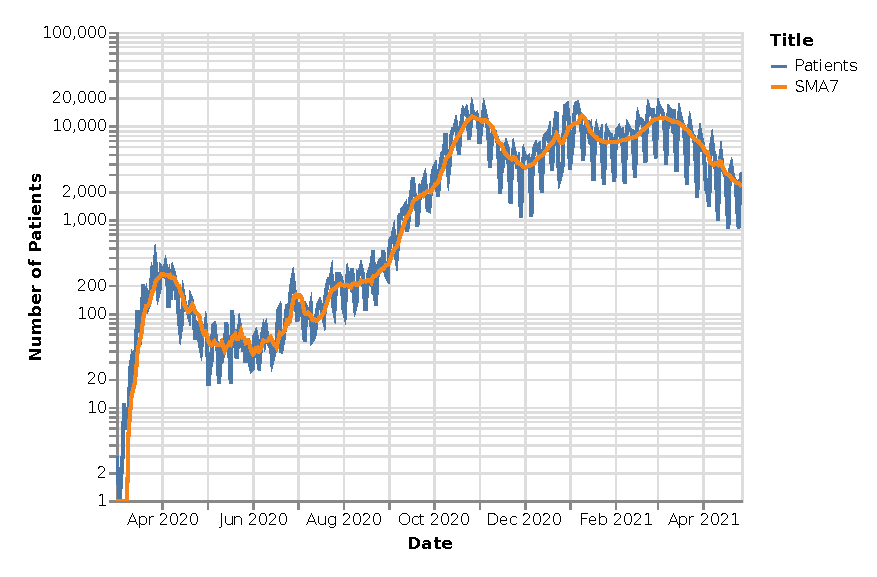
\includegraphics[width=0.9\textwidth]{figures/recovered-sma7.eps}
    \caption{Daily confirmed cases of infection and weekly moving average.}
    \label{fig:recovered-sma7}
\end{figure}
\FloatBarrier

\section{Summary}

The possibilities of analysis of the selected data set are limited and determining their quality is very difficult.
The main reason for the difficulties is the nature of the data, which corresponds in structure to econometric data, already processed in a certain way.
Thus, an available data catalog is in practice a set of results without background data.
Moreover, we tried to draw conclusions from existing data and tried to learn their quality without knowledge of the criterial limitations and general description of the data, which should be determined by the methodological guideline.
However, the instructions providing the necessary information about the data is missing (or is insufficiently informative) in these cases.
